%!TEX root = main.tex

\section{Preliminaries}\label{sec:prel}

Throughout the paper, $\Int^+$ denotes the set of positive integers, and  $\nat$ denotes the set of natural numbers. Furthermore, for $n\in \Int^+$, let $[n]:=\{1, \ldots, n\}$. 

We use $\Sigma$ to denote a finite set of letters, called \emph{alphabet}. A \emph{string} over $\Sigma$ is a finite sequence of letters from $\Sigma$. We use $\Sigma^*$ to denote the set of strings over $\Sigma$. A string $w'$ is called a \emph{prefix} of $w$ if $w = w'w''$ for some string $w''$. We use $\pref(w)$ to denote the set of prefixes of $w$. For a prefix $w_1$ of $w$, let $w = w_1 w_2$, then we use $w_1^{-1}w$ to denote $w_2$.

\begin{definition}[Finite-state automata] \label{def:nfa}
	A \emph{(nondeterministic) finite-state automaton}
	(\FA{}) over a finite alphabet $\ialphabet$ is a tuple $\Aut =
	(\ialphabet, \controls, q_0, \finals, \transrel)$ where 
	$\controls$ is a finite set of 
	states, $q_0\in \controls$ is
	the initial state, $\finals\subseteq \controls$ is a set of final states, and 
	$\transrel\subseteq \controls \times 
	\ialphabet \times  \controls$ is the
	transition relation. 
\end{definition}

For an input string $w=a_1 \dots a_n$, a \emph{run} of $\Aut$ on $w$
%(with $a_0 = \EndLeft$ and $a_{n+1} = \EndRight$)
is a sequence of states $q_0, \ldots, q_n$ such that $(q_{j-1}, a_{j}, q_{j}) \in
\transrel$  for every $j \in [n]$.
The run is said to be \defn{accepting} if $q_n \in \finals$.
A string $w$ is \defn{accepted} by $\Aut$ if there is an accepting run of
$\Aut$ on $w$. In particular, the empty string $\varepsilon$ is accepted by $\Aut$ if $q_0 \in F$. The set of strings accepted by $\Aut$, i.e., the language \defn{recognised} by $\Aut$, is denoted by $\Lang(\Aut)$.
%Since we deal with computational complexity in the sequel, we define
The \defn{size} $|\Aut|$ of $\Aut$ is defined to be the cardinality of the set $Q$ of states, which will be 
used when the computational complexity is concerned.

For convenience, for $a \in \Sigma$, we use $\delta^{(a)}$ to denote the  relation $\{(q, q') \mid (q, a, q') \in \delta\}$.


  
%%%%%%%%%%%%%%%%%%%%%%%%%%%%%%%%%
 \subsection{Extended regular expressions}
%%%%%%%%%%%%%%%%%%%%%%%%%%%%%%%%%%  
An (extend) regular expression (with capturing group and back reference) is defined as follows.
  
\begin{definition}[Regular expressions with capturing group and back reference, $\regexp$]
  	\[e \eqdef \emptyset \mid \varepsilon \mid a \mid \$n \mid e + e \mid e \concat e \mid e^* \mid e^{*?} \mid (e)  , \]
  	where $a \in \Sigma, n \in \Int^+$. 
  	%	Since $+$ is associative and commutative, we also write $(e_1 + e_2) + e_3$ as $e_1 + e_2 + e_3$ for brevity. 
  	%We use the abbreviation 
\end{definition}
We abbreviate $e \concat e^*$ as $e^+$ and $e \concat e^{*?}$ as $e^{+?}$. Moreover, for $\Gamma = \{a_1, \ldots, a_k\}\subseteq \Sigma$, we write $\Gamma$ for  $a_1 + \cdots + a_k$ and thus  $\Gamma^\ast \equiv (a_1 + \cdots + a_k)^\ast$. 

Note that the parentheses in $\regexp$ are used for both precedence and capturing groups. 
%We assume that the parentheses in every regular expression are well matched. 
%
%Besides the common rules governing regular expressions, a regex obeys
%the following syntactic rule: 
Parenthesis pairs are indexed according to the occurrence sequence of their left parentheses, and it is required that every back reference $\$ n$ occurs  %the right of 
after the $n$-th pair of parentheses. For instance, $((a+b)^*) c \$1$ is in $\regexp$, where $\$1$ refers to the matching of the subexpression $(a+b)^*$. Intuitively, it denotes the set of strings of the form $u c u$, where $u$ is a string of $a$ and $b$. 
%with each letter being $a$ or $b$.
  
%Note that standard regular expressions are those without $\$ n$. 
%Moreover, 
We use $\regexp[\sf CG]$ to denote the fragment of $\regexp$  excluding $\$ n$, and $\refexp$ to denote the set of expressions generated by $e \eqdef \varepsilon \mid a \mid \$n \mid e \concat e$.
  %\tl{define the semantics here?}
  
  %\label{semantics:regex}
  
  
  
  %\subsection{Semantics of \regexp[\sf CG]}
  %In this section, we give one of the many semantics of \regexp[\sf CG], which we will utilize for $\replaceall$.
  
  \begin{definition}[Subexpression]
  	For any two $\regexp$ $e$ and $r$, we say $r$ is a subexpression of $e$,
  	if either $r=e$ or
  	\begin{itemize}
  		\item If $e = e_1 e_2$ or $e_1 + e_2$ then $r$ is a subexpression of $e_1$
  		or $e_2$
  		
  		\item If $e = e_1^{\ast}$, $e_1^{\ast?}$, or $(e_1)$, then $e_1$ is a subexpression of $e$.
  	\end{itemize}
  	We use $S (e)$ to denote the set of all subexpressions of $e$.
  \end{definition}

We  define the semantics of $\regexp$, which uses a concept of matches of $e \in \regexp$ to strings $w$ defined in the sequel.
  
  \begin{definition}[Match of $\regexp$ to strings]
  	A \tmtextbf{match} of $\regexp$ $e$ to a string $w$ is defined by a finite directed and ordered
  	tree $T$, whose nodes are elements of $\Sigma^{\ast} \times S (e)$ satisfying the following constraints: Its root is $(w, e)$, and for any node $\alpha =
  	(w', e')$ in $T$, we have:
  	\begin{itemize}
  		\item If $e' = e'_1 \concat e'_2$, then $\alpha$ has two children $\alpha_1 = (w'_1,
  		e'_1)$ and $\alpha_2=(w'_2, e'_2)$ where $w' = w'_1 w'_2$.
  		
  		\item If $e' = e'_1 + e'_2$, then $\alpha$ has a single child $\alpha_1 = (w',
  		e'_i)$ where $i \in \{ 1, 2 \}$.
  		
  		\item If $e' = {e'_1}^{\ast}$ or ${e'_1}^{\ast ?}$, then either $w' = \varepsilon$ in which case $\alpha$ is a
  		leaf, or there is $k \geqslant 1$ such that $\alpha$ has $k$ children $\alpha_1 = (w'_1,
  		e'_1), \ldots, \alpha_k = (w'_k, e'_1)$ where $w' = w'_1 \ldots w'_k$ and for all
  		$i \in [k]$, $w'_i \neq \varepsilon$, (even if $\varepsilon \in L
  		(e'_1)$).
%
%  		\item If $e' = {e'_1}^{\ast?}$, then either $w' = \varepsilon$ in which case $\alpha$ is a
%  		leaf, or there is $k \geqslant 1$ such that $\alpha$ has $k$ children $\alpha_1 = (w'_1,
%  		e'_1), \ldots, \alpha_k = (w'_k, e'_1)$ where $w' = w'_1 \ldots w'_k$ and for all
%  		$i \in [k]$, $w'_i \neq \varepsilon$ (even if $\varepsilon \in L
%  		(e'_1)$).
%  		\tl{what is the difference?}
%		
  		\item If $e' = (e'_1)$, then $\alpha$ has a single child $\alpha_1 = (w', e'_1)$.
 % 		
  		\item If $e' = a$ (resp. $e' = \varepsilon$), then $\alpha$ is a leaf and
  		$w' = a$ (resp. $w' = \varepsilon$).
%		
		\item If $e' = \$n$, then $\alpha$ is a leaf of $T$, moreover, let $e'' \in S(e)$ be enclosed by the $n$-th pair of parentheses in $e$ and $\beta = (w_1, e_1)$ be the last node preceding $\alpha$ in $T$ such that $e_1 = e''$, according to the left-to-right ordering of the nodes, then $w' = w_1$.
  	\end{itemize}
  	
%  	Whenever unambiguous, we use a node u to represent the whole subtree
 We use $T_\alpha$ to represent the subtree of $T$ rooted at $\alpha$.
 % 	where u is the root. 
The notation $C(T)$ refers to the sequence of direct children of the root node of $T$ (and thus all direct subtrees).
%
%If a tree $T$ is a match of $e$ to a string $w$, then it is called a \emph{match tree} of $e$ \tl{to $w$?}. 
We use $\cM_{w}(e)$ to denote the set of all match trees of $e$ to $w$. Moreover, for $L \subseteq \Sigma^\ast$, we use $\cM_{L}(e)$ to denote the set of match trees of $e$ to some $w \in L$.
We also use $\Lang(e)$ to denote $\{w \in \Sigma^* \mid \cM_w(e) \neq \emptyset\}$. 
  \end{definition}
  
  \begin{definition}[Semantics of $\regexp$]\label{def-regex-semantics}
  		
  	For any $\regexp$ $e$ and a string $w$, we recursively define a total order on $\cM_{\pref(w)}(e)$, written $T
  	>_{w,e} T'$, where $T, T' \in \cM_{\pref(w)}(e)$, as follows:
  	\begin{itemize}
  		\item $e = \varepsilon$ or $e = a$ or $e = \$ n$. There is only one match tree, thus the
  		order $>_{w, e}$ is empty.
  		
  		\item $e = (e_1)$. Suppose that $C (T) = (w_1, e_1)$ and $C (T') = (w_2, e_1)$ for some $w_1, w_2 \in \pref(w)$.
  		Then $T >_{w,e} T'$ iff $T_{(w_1, e_1)} >_{w, e_1} T'_{(w_2, e_1)}$.
  		
  		\item $e = e_1 + e_2$.
  		\begin{itemize}
  			\item If $C (T) = (w_1, e_1)$ and $C (T') = (w_2, e_2)$ for some $w_1, w_2 \in \pref(w)$, then $T >_{w,e} T'$.
%  			
  			\item If $C (T) = (w_i, e_i)$ and $C (T') = (w'_i, e_i)$ for some $i \in \{ 1,
  			2 \}$ and $w_i, w'_i \in \pref(w)$, then $T >_{w,e} T'$ iff $T_{(w_i, e_i)} >_{w, e_i} T'_{(w'_i, e_i)}$.
  		\end{itemize}
  		\item $e = e_1 \cdot e_2$. Suppose $C (T) = (w_1, e_1) (w_2, e_2)$ and $C (T') =
  		(w_1', e_1) (w_2', e_2)$, then $T >_{w,e} T'$ when either $T_{(w_1, e_1)} >_{w, e_1}
  		T'_{(w_1', e_1)}$, or $w_1 = w_1'$ and $T_{(w_2, e_2)} >_{w_1^{-1}w, e_2} T'_{(w_2', e_2)}$.
%  		
  		\item $e = e_1^{\ast}$. 
		\begin{itemize}
		\item If $T' $ is  a single node $(\varepsilon, e)$, but $T$ is not, then $T >_{w, e} T'$.
  		\item Otherwise, suppose $C(T) = (w_1, e_1) \ldots (w_k, e_1)$ and $C (T') =
  		(w_1', e_1) \ldots (w_l', e_1)$, we have $T >_{w,e} T'$ iff either when $C (T')$
  		is a proper prefix of $C (T)$, or for the first index $j$ such that $w_j
  		\neq w_j'$, we have $T_{(w_j, e_1)} >_{(w_1\cdots w_{j-1})^{-1}w, e_1} T'_{(w_j', e_1)}$.
		\end{itemize}
%
  		\item $e = e_1^{\ast?}$. 
		\begin{itemize}
		\item If $T$ is  a single node  $(\varepsilon, e)$, but $T'$ is not, then $T >_{w, e} T'$.
  		\item Otherwise, suppose $C(T) = (w_1, e_1) \ldots (w_k, e_1)$ and $C (T') =
  		(w_1', e_1) \ldots (w_l', e_1)$, we have $T >_{w,e} T'$ iff either when $C (T)$
  		is a proper prefix of $C (T')$, or for the first index $j$ such that $w_j
  		\neq w_j'$, we have $T_{(w_j, e_1)} >_{(w_1\cdots w_{j-1})^{-1}w, e_1} T'_{(w_j', e_1)}$.
		\end{itemize}
  	\end{itemize}
  	
  	For $e \in \regexp$ and $w \in \Lang(e)$, the \emph{accepting match} of $e$ to $w$, denoted by $M_e(w)$, is the supremum of $\cM_w(e)$. Moreover,  for $e \in \regexp$ and $w \in \Sigma^\ast$, if there is $w \in  \Sigma^\ast\Lang(e)\Sigma^\ast$, then the (first) \emph{match} of $e$ in $w$ is defined as the accepting match of $e$ to $w'$ such that $w = w_1w'w_2$ for some $w_1,w_2\in \Sigma^\ast$ and for every nonempty suffix $w'_1$ of $w_1$, $w'_1w'w_2 \not \in \Lang(e)\Sigma^\ast$, otherwise, the match of $e$ in $w$ is undefined.  
%  	
%  	For any subexpression $e'$ of $e$, suppose $(w_1, e') \ldots (w_m, e')$ are
%  	all the nodes labeled by $(w', e')$ with $w' \neq \varepsilon$, in the
%  	pre-order traversal of $M_e(w)$. Then the match result captured by $e'$, denoted
%  	by $M_{e', e} (w)$, is the sequence of substrings $w_1 \ldots w_m$.
  \end{definition}

\begin{example}\label{exmp-regex-semantics}
Let $e = ((b^\ast) \cdot ((b \cdot a^\ast) | \varepsilon)) \cdot a^\ast$ and $w= baa$. Then $\cM_{w}(e) = \{T_1,T_2,T_3\}$ as illustrated in Figure~\ref{fig-regex-semantics}: (i), (ii), (iii).  Because  $(T_2)_{(\varepsilon, b^\ast)}$ is a single node, while $(T_1)_{(b,b^\ast)}$ is not, we have $(T_1)_{(b,b^\ast)} >_{w, b^\ast} (T_2)_{(\varepsilon, b^\ast)}$, thus $(T_1)_{(b, (b^\ast))} >_{w, (b^\ast)} (T_2)_{(\varepsilon, (b^\ast))}$. From the fact that $(T_1)_{(b, (b^\ast))}$ and $(T_2)_{(\varepsilon, (b^\ast))}$ are the left subtrees of $(T_1)_{(b, (b^\ast) \cdot ((b\cdot a^\ast) | \varepsilon))}$ and $ (T_2)_{(ba, (b^\ast) \cdot ((b\cdot a^\ast) | \varepsilon))}$ respectively, we deduce that $(T_1)_{(b, (b^\ast) \cdot ((b\cdot a^\ast) | \varepsilon))} >_{w, (b^\ast) \cdot ((b\cdot a^\ast) | \varepsilon)} (T_2)_{(ba, (b^\ast) \cdot ((b\cdot a^\ast) | \varepsilon))}$, thus $(T_1)_{(b, ((b^\ast) \cdot ((b\cdot a^\ast) | \varepsilon)))} >_{w, ((b^\ast) \cdot ((b\cdot a^\ast) | \varepsilon))} (T_2)_{(ba, ((b^\ast) \cdot ((b\cdot a^\ast) | \varepsilon)))}$. From this, we conclude that $T_1 >_{w, e} T_2$. Similarly, we have $T_1 >_{w, e} T_3$. Therefore, $M_e(w) = T_1$. 
Note that in $T_1$, the capturing group $((b^\ast) \cdot ((b\cdot a^\ast) | \varepsilon))$ does not acquire the longest match. Moreover, the match of $e$ in $baabba$ is $baa$, where the matches of the first and second capturing group are $b$ and $\varepsilon$ respectively, while the match of the third capturing group is undefined.
\begin{figure*}[ht]
\centering
%\rule{\linewidth}{0cm}
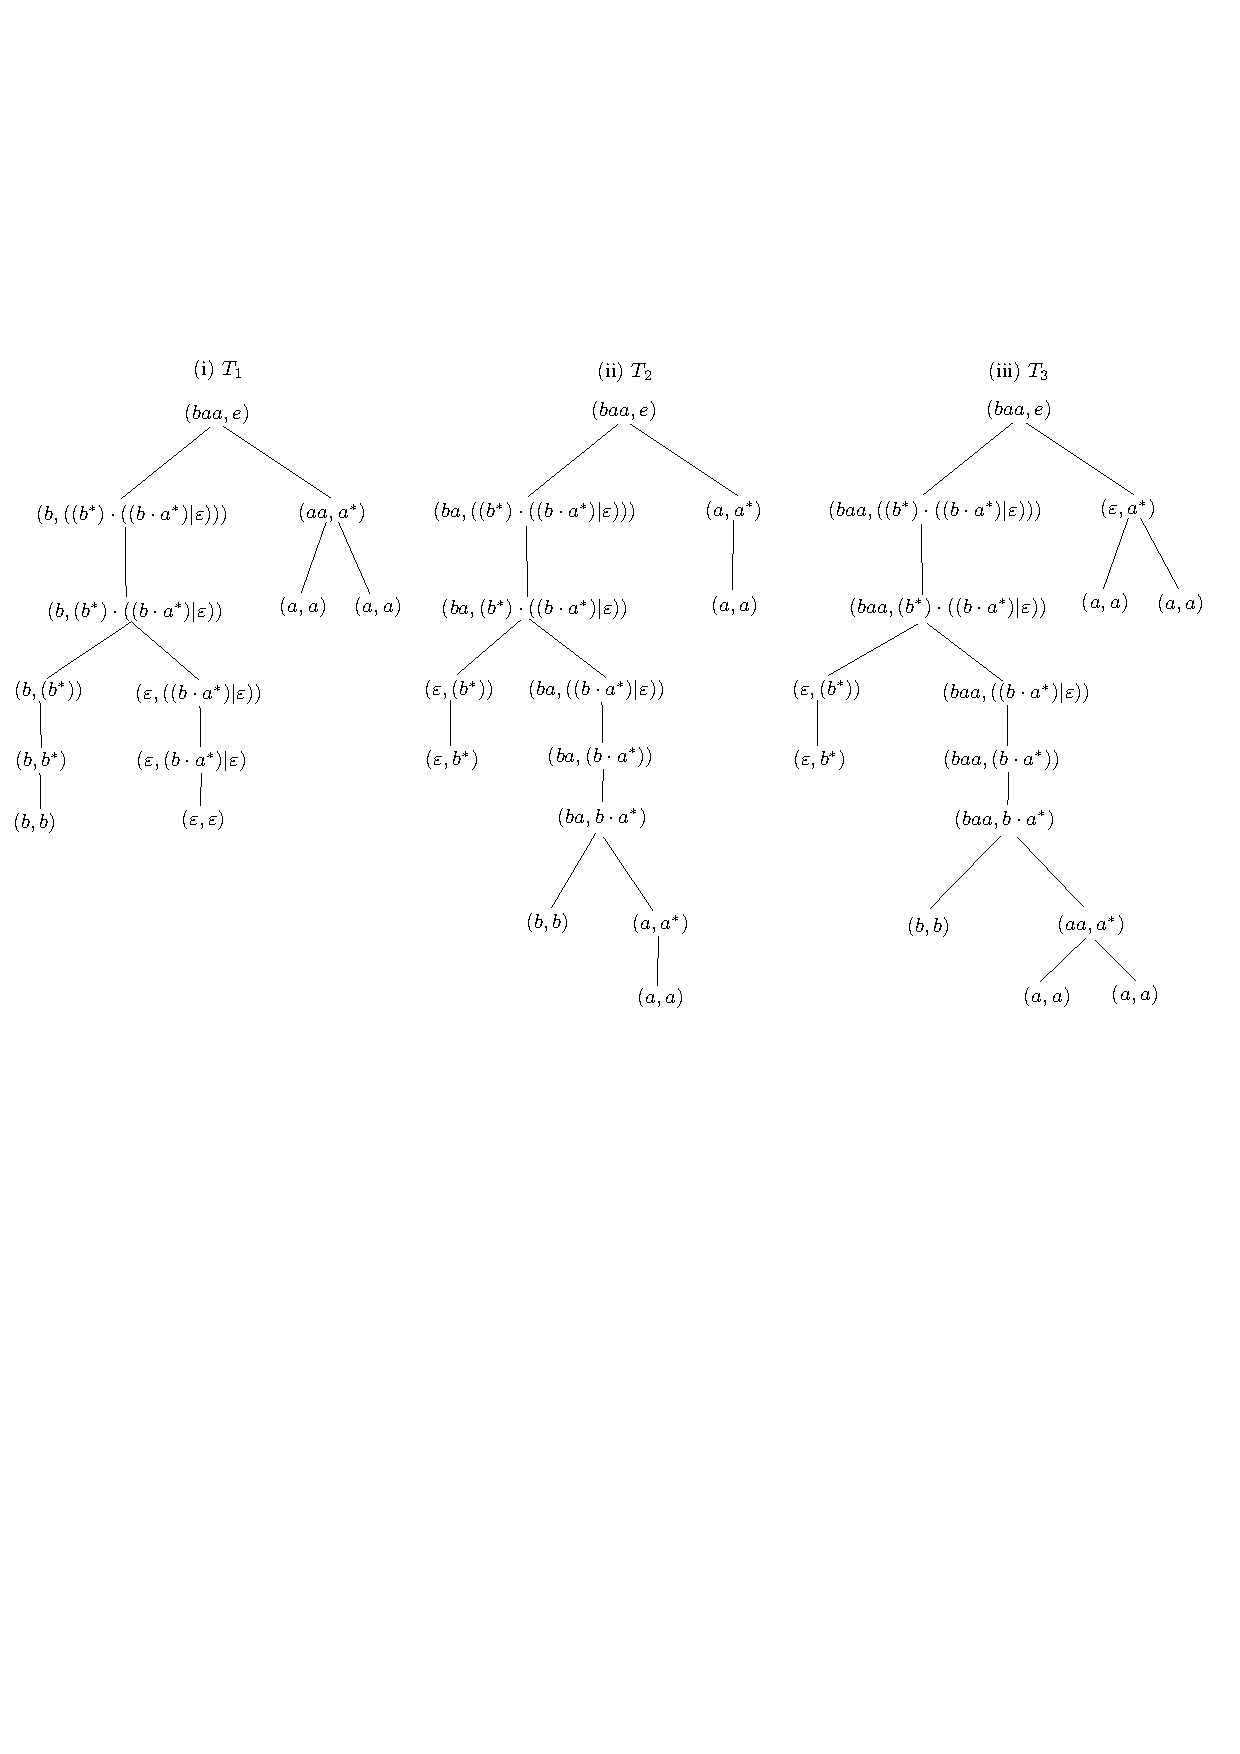
\includegraphics[scale=0.7]{regex-semantics.pdf}
\caption{Match trees of $e=((b^\ast) \cdot ((b \cdot a^\ast) | \varepsilon)) \cdot a^\ast$ to $w= baa$}
\label{fig-regex-semantics}
\end{figure*}
%\Blindtext
 \end{example}
  
\begin{remark}
Intuitively, the semantics of $\regexp$ in Definition~\ref{def-regex-semantics} is eager for $e_1 + e_2$ and greedy for $e^\ast$, which is adopted by the script languages Perl, PHP, and Javascript etc \cite{MasterREbook}. In comparison, POSIX regular expressions require the leftmost and longest match, of which we leave the investigation as the future work. 
\end{remark}
  
  
% some examples
  
%  e = b(a*)a*
%  
%  e' = b(a*?)a*
